\chapter{Recursive Make}
\label{chap:rMake}

When software development projects grow bigger is it not uncommon that the different source files are spread over multiple folders. And even those folders can contain subfolders with even more source files.

Compiling such big projects can be a hassle. If you put everything in a single Makefile, this will result in a (very) big file. For this reason was it common practise to have in every subfolder a Makefile (see figure \ref{fig:recmake_project}) and in the Makefile of the parent folder a loop to start in every subfolder a new make instance. This give however several issues with incomplete recompilations and very slow compiling.

 \begin{figure}[H]
  \centering
  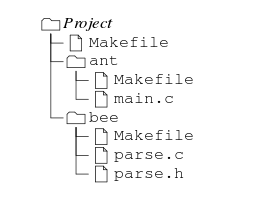
\includegraphics[width=5cm]{Images/recmake-project.png}
  \caption{ Example project with multiple modules with their own Makefile.}
  \label{fig:recmake_project}
\end{figure}

In 1997 a paper \cite{recmake} was published that proposed a different solution that would also solve the issues with incomplete and slow (re)compilation. The source of all the common issues with make was that the Makefile didn't provide a complete image of the work to do. This combined with re-doing certain steps for every Makefile resulted in the situation mentioned. Such full graph is showed in figure \ref{fig:recmake_fullgraph}.

\begin{figure}[H]
  \centering
  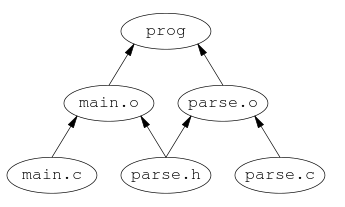
\includegraphics[width=5cm]{Images/makerec-fulll-graph.png}
  \caption{ Full graph of the dependencies in the project. }
  \label{fig:recmake_fullgraph}
\end{figure}

\begin{figure}
  \centering
  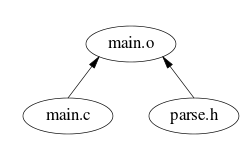
\includegraphics[width=5cm]{Images/makerec-graph-main.png}
  \caption{ Make graph for the ant subfolder. }
  \label{fig:recmake_graph-main}
\end{figure}

Make creates a graph of the different targets (see figure \ref{fig:recmake_graph-main} and \ref{fig:recmake_graph-bee}) and determines with it the work it should do. If however the graph is incomplete, for example because certain source files are in a different subfolder and managed by a different Makefile, the recompilation of the project could be incomplete. Make simply doesn't know about the other dependencies.


\begin{figure}[H]
  \centering
  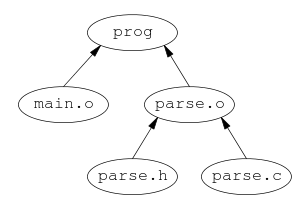
\includegraphics[width=5cm]{Images/makerec-bee-graph.png}
  \caption{ Make graph for the bee subfolder. }
  \label{fig:recmake_graph-bee}
\end{figure}

In the situation situation of figure \ref{fig:recmake_graph-bee} this is not a problem, however it is when there is for example a cyclic dependency or when on the dependency's in the ant folder is generated (like in figure \ref{fig:recmake_graph-bee2}) by a step with the Makefile of the bee folder. In this case parse.h is generated by a build step with parse.y. The graph of the ant folder however would remain the same. This means main.c is not recompiled after parse.h is regenerated. 

\begin{figure}
  \centering
  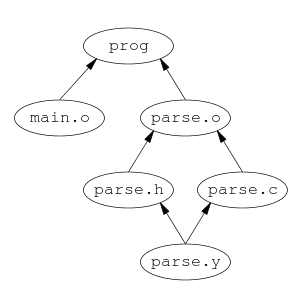
\includegraphics[width=5cm]{Images/makerec-bee2-graph.png}
  \caption{ Make graph for the bee subfolder in the case that parse.h and parse.c are generated by another dependency. }
  \label{fig:recmake_graph-bee2}
\end{figure}